\chapter{Results \& Discussion}

\textbf{Should include a reiteration of the experiments, and their outcome.  Together with a description (discussion).  Preamble should include a reminder of the aims and objectives together with a list of experiments to achieve these.  Should include many charts and other visualization with appropriate descriptions}.  


\section{Determining the Optimal Tools}

The following is the reasoning behind the final decisions made on the tool choices of each step of the pipeline, based on the literature reviewed in Section \ref{Computational Tools}. Extensive descriptions of the final tools implemented in the pipeline can be found throughout Section \ref{RNA-seq: in silico}.
% NOTE SEE IF U NEED TO CHANGE THIS. Maybe group all the tools in a single place

Tools which measure quality metrics without altering the data require little justification for their use, their mention occasionally being completely omitted from RNA-seq studies (\autoref{tab:rnaseq_experiments}). \textbf{FastQC} is a staple of sequencing quality control, providing a detailed analysis of the contents of FASTQ files and drawing attention to signs of low quality reads. While FastQC results are detailed, they lack the detection of external nucleotide contaminants in the data. This information was supplemented with the results from \textbf{FastQScreen} which aligns the experimental sequences to common contaminant sequences (e.g. mouse, \textit{Drosophila}, rRNA) and provides a graph marking any successful alignments.

\cite{he2020assessing} found that the effects of their tested preprocessing techniques on downstream analyses are marginal, thus we base our decision on the frequency of the tools used in tables \ref{tab:rnaseq_experiments} and \ref{tab:packaged_pipelines} and their functionality. \textbf{Cutadapt} adequately satisfies these criteria, providing the means to trim adapter sequences and remove short reads. \textbf{Trim Galore!} pipes the output to FastQC, which facilitates the reassessment of quality. To complement their functionality, \textbf{Prinseq++} was chosen to detect and remove regions of low-complexity which were noticeably neglected in studies' preprocessing steps. 
%\cite{liao2020read} and \cite{he2020assessing} doubt the necessity of trimming at all.

Despite \textbf{STAR} being demanding of RAM \citep{Dobin2013} and slower than more light-weight aligners \citep{srivastava2020alignment}, these were not limiting factors due to our access to a High Performance Computer (HPC) and small number of samples. \cite{srivastava2020alignment} found that the choice between quasi-mappers (e.g. Salmon) and traditional aligners (e.g. STAR) is a trade-off between speed and accuracy. Similarly \cite{Zhang2017} found that pseudo-aligners Salmon and Kallisto require less runtime while maintaining similar accuracy to STAR. \cite{Schaarschmidt2020} find that the effect aligners have on the final list of \ac{DEG}s is negligible, and that all tested aligners can be used equally for RNA-seq. Even if STAR provides a marginal increase in accuracy over quasi-aligners, this is preferable over the improvements in speed or computational demand provided by other aligners.

An RNA-seq quantification tool benchmark, \cite{teng2016benchmark}, conclude that their tested tools performed similarly, with the exception of the under-performing Flux Capacitor \citep{} and eXpress \citep{}. \textbf{RSEM} was amongst these tools, and was ultimately chosen on the basis of its statistical techniques based on \cite{li2010rna} to mitigate ambiguous read alignment. Its support for the STAR aligner is also convenient, allowing the combination of alignment and quantification steps. 


\subsection{Adapting DGE Analysis to a Lack of Replicates}
\label{DGE no replicates}

The most difficult and time-consuming decision to make was the choice of tool to perform \ac{DGE} analysis. The invested effort was justified by the findings of \cite{williams2017empirical}, which state that the method of \ac{DGE} exhibits the strongest impact on the results out of all stages of the pipeline. Our data consists of three time points (1hr, 6hr, 12hr) and a negative control, each lacking replicates. 

Technical replicates allow the isolation of the non-biological variation to evaluate the quality of the instruments and methodology used. By contrast, biological replicates originate from different biological sources and are meant to test the biological variance of the samples. \cite{liu2014rna} find that in RNAseq biological variation is by far more important, and given a choice between the two, the researcher should invest in biological replicates. \cite{bullard2010evaluation} confirm this claim, finding that technical variation in RNAseq experiments is minimal. \cite{schurch2016many} found that using three biological replicates gave 20\% to 40\% of the \ac{DEG}s (varies according to the tool) compared to a full set of 42 replicates (representing the 'true' population). This rises to >85\% when considering genes with a log$_2$ fold change of >2. \cite{schurch2016many} state that ideally an RNAseq experiment for \ac{DGE} should have a minimum of six replicates per condition for all experiments and 12 replicates for experiments where the identification of \textit{all} the \ac{DEG}s, even the lowly expressed ones, is important. 

However, in practice, performing an experiment with large numbers of replicates is not always possible. Budget constraints and the still-high cost of sequencing are a common issue in RNAseq experiments. One may argue that this issue is mitigated due to the negligible technical variance of RNA-seq \citep{bullard2010evaluation} and the minimal biological variance in samples from the same \ac{ATRA}-resistant HL-60 cell line. In spite of this, the statistical tests used by conventional \ac{DGE} tools are dependent on the calculation of the variance or dispersion, which is not mathematically possible with a single reading per condition. To make the most of such datasets, several \ac{DGE} tools advertise their ability to work with just a single reading per experimental condition \citep{feng2012gfold, gim2016lpeseq, anders2010differential, wang2010degseq, al2014bootstrap}. Notably, DESeq2 does not support datasets without replicates. There is an unfortunate lack of review papers and independent studies which benchmark these tools. For this reason this section will be reviewing the available tools adapted to performing \ac{DGE} without replicates.

The first tool in this review will be \textbf{GFOLD} \citep{feng2012gfold}, developed specifically for datasets lacking in replicates. The developers acknowledge the dependence of \textit{p}-values on variance estimation, which is impossible without replicates. A unique GFOLD value replaces the standard metrics of significance (\textit{p}-values) and expression change (log$_2$ fold changes). \cite{feng2012gfold} describe the value as a relative change of the expression level. GFOLD is unique in that it is the only tool in this comparison that is called through the Linux command line, instead of being an R library.

\textbf{LPESeq} \citep{gim2016lpeseq} introduces the Local-Pooled-Error (LPE) method for few or single-replicate \ac{DGE} analysis. This method attempts to estimate transcript-specific variance using the raw values of each transcript per condition. Hypothesis testing for significant difference is then performed to identify the differentially expressed genes.

\textbf{IsoDE} \citep{al2014bootstrap} is a non-parametric method (i.e. it assumes no statistical distribution) and is based on bootstrapping. The algorithm generates FPKM estimates from read counts of each condition which undergo pairwise comparison.

An MA-plot-based method, the R library \textbf{DEGseq} \citep{wang2010degseq} (not to be confused with DESeq) accepts input .bed or .eland input files and outputs an XHTML page with \textit{p}-values, gene expression values and expression differences in the form of Q-values.

The final tool in this review is the Bioconductor R library \textbf{edgeR} \citep{edger}. It may be more accurately described as a collection of methods, neither of which are specifically adapted to data without replicates, but its documentation provides recommendations to adapt the analysis to such a situation. EdgeR and its normalisation technique TMM have already been covered extensively in Section \ref{EdgeR} and Section \ref{TMM} respectively. 

The lesser-known tools (GFOLD, LPESeq, DEGseq, IsoDE), while developed specifically to function without replicates, were found to be limited in functionality in comparison to \textbf{edgeR}. Additionally, due to their rather unconventional approach to \ac{DGE}, their output was found to be incompatible with other downstream libraries, limiting the potential for data exploration. 

EdgeR has multiple methods to determine which genes are differentially expressed (\autoref{edger_dge_options}). The likelihood ratio tests \citep{mccarthy2012differential} compared values against their mean, which was not applicable to our study as we needed to compare reads from treated cells against reads from untreated cells. Quasi-likelihood F-tests \citep{lun2016s, lund2012detecting} were simply not compatible to datasets lacking replicates. This leaves us with the \textit{classic} approach: the exact test for the negative binomial distribution \citep{robinson2007moderated, robinson2008small}. This is a pairwise test which compares the means between two groups of counts, applicable to experiments with a single factor. It should not be confused with Fisher's exact test \citep{fisher1922interpretation}, although the two share a number of similarities \citep{chen2014edger}. 

The exact test for the negative binomial distribution still involves the calculation of dispersion of the data, but the edgeR vignette suggests a method to circumvent this. It suggests nominal values for the biological variation (\ac{BCV}) of our data based on previous experiments, from which we may derive an estimation for the dispersion. The vignette emphasises that this method is still inaccurate, but was deemed as the best possible solution given our data and the aforementioned potential techniques. 
% WRITE ABOUT RSEM AND MULTIQC

% really perfect paper https://www.ncbi.nlm.nih.gov/pmc/articles/PMC4878611/#:~:text=Recommendations%20for%20RNA%2Dseq%20experiment%20design&text=At%20least%20six%20replicates%20per,all%20DE%20genes%20is%20important.


\section{Quality Control}
This section encompasses all QC measures taken prior to differential expression analysis. MultiQC is able to read and compile log files from FastQC, FastQScreen, Cutadapt and STAR into a single interactive HTML file, allowing quality comparisons across samples. Figures \ref{fig:fastqc-status-check-heatmap} through \ref{fig:star_alignment_plot} are graphs downloaded directly from MultiQC.


\subsection{Assessing the Quality of the Raw Data}
\label{Assessing the Quality of the Raw Data}
We started off with four single-ended 50bp FASTQ files, one per experimental time point (control, 1hr, 6hr, 12hr), which were sequenced using the Illumina Stranded mRNA-seq workflow \citep{HiSeq2000}. Paired-end reads of a longer length would have been more accurate, although on their website\footnote{Accessed 16/06/22: \url{https://emea.illumina.com/science/technology/next-generation-sequencing/plan-experiments/read-length.html}}, Illumina suggests that single-ended 50bp reads suffice for a \ac{DGE} RNA-seq experiment.

\autoref{fig:fastqc-status-check-heatmap} shows the FastQC results for each raw file, summarised as a heatmap generated by MultiQC. Caution should be exercised when interpreting RNA data through FastQC, as the program is primarily calibrated to DNA data. Two modules failed consistently throughout the four samples received. This is normal and expected even for high-quality RNA \citep{hansen2010biases}. The failure of the \textit{Per base sequence content} module can be explained by a benign artefact of the random hexamer priming that occurs during library preparation, where the first 10-15 bases of RNA reads are non-uniformly enriched \citep{hansen2010biases}. The failure for the second module, textit{Sequence Duplication Levels} is explained by \autoref{fig:fastqc_sequence_duplication_levels_plot} and the text preceding it.

All four samples had <0.3\% \textit{N}-content on average on the first base of the reads and <0.1\% on the rest of the read, which the algorithm deems as good quality. All sequences of all samples had a single length of 51bp with <1\% overrepresented sequences and <0.5\% adapter contamination.

%Write about terminator caps in intro

% https://hbctraining.github.io/Intro-to-rnaseq-hpc-salmon/lessons/qc_fastqc_assessment.html
% Really good resource on RNAseq QC
 %Another one: https://rtsf.natsci.msu.edu/genomics/tech-notes/fastqc-tutorial-and-faq/#:~:text=FastQC%2C%20written%20by%20Simon%20Andrews,on%20a%20sequence%20data%20set.


% INTERNPRETING FASTQC REPORT NOTES:
% Real good resource of possible explanations:
% We have positional sequence bias: https://sequencing.qcfail.com/articles/positional-sequence-bias-in-random-primed-libraries/
% High Sequence Duplication levels are expected: https://www.biostars.org/p/307361/
%From Molecular Biology assignment:
%  One cycle per base pair would have been needed, so 50 cycles should have been performed.


\newpage
\begin{figure}[!h]
    \centering
    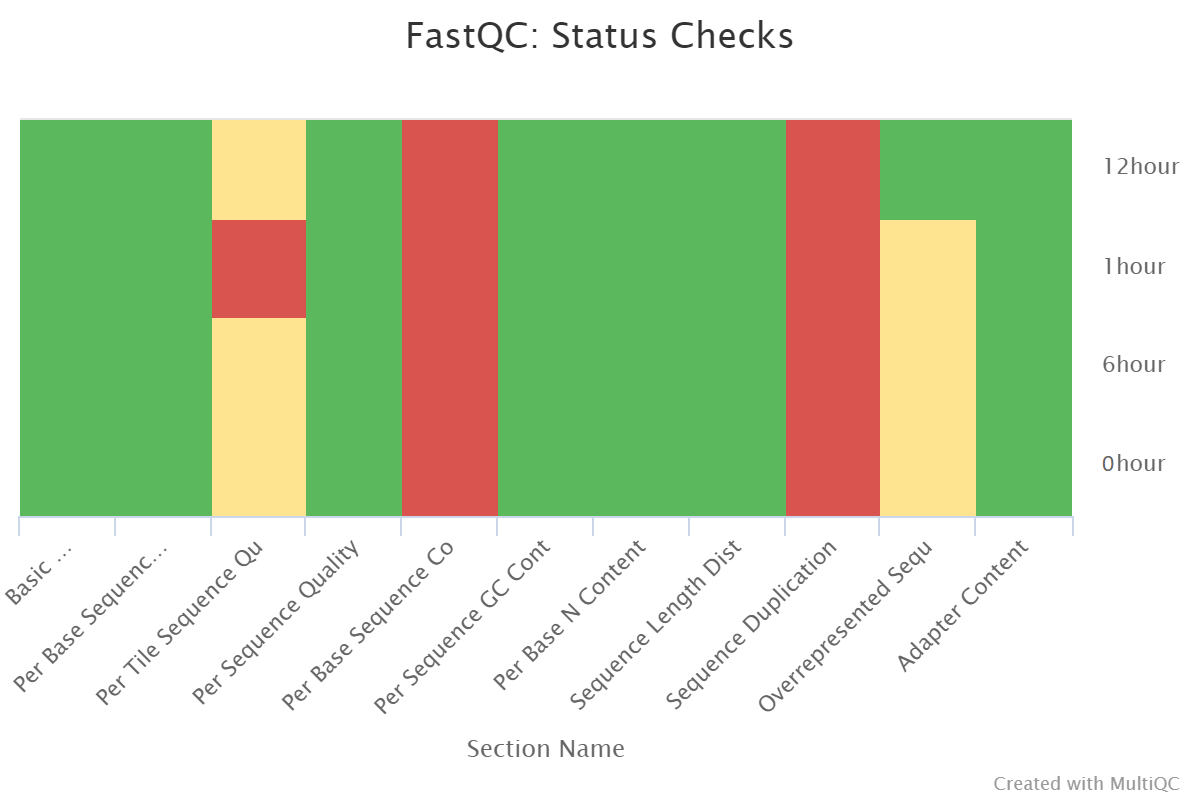
\includegraphics[width=1\textwidth]{fastqc-status-check-heatmap}
    \caption[Heat map showing the status of each FastQC module]{Heat map generated by MultiQC showing the status of each FastQC module: Pass, Warning or Fail.} 
    \label{fig:fastqc-status-check-heatmap}
\end{figure}

\newpage
Part of the sequencing process involved PCR amplification of cDNA, although not all sequences are amplified equally \citep{kozarewa2009amplification}. These PCR duplicates differ from 'natural' duplicates, i.e. those that originated from different mRNA molecules. Both these factors contribute to certain sequences being disproportionately abundant (as seen in \autoref{fig:fastqc_sequence_duplication_levels_plot}), which FastQC flags as duplicates, causing the failure of the \textit{Sequence Duplication Levels} module. \cite{parekh2016impact} state that there is no clear consensus on what should be done with these duplicates, with their removal producing conflicting results.

\begin{figure}[!h]
    \centering
    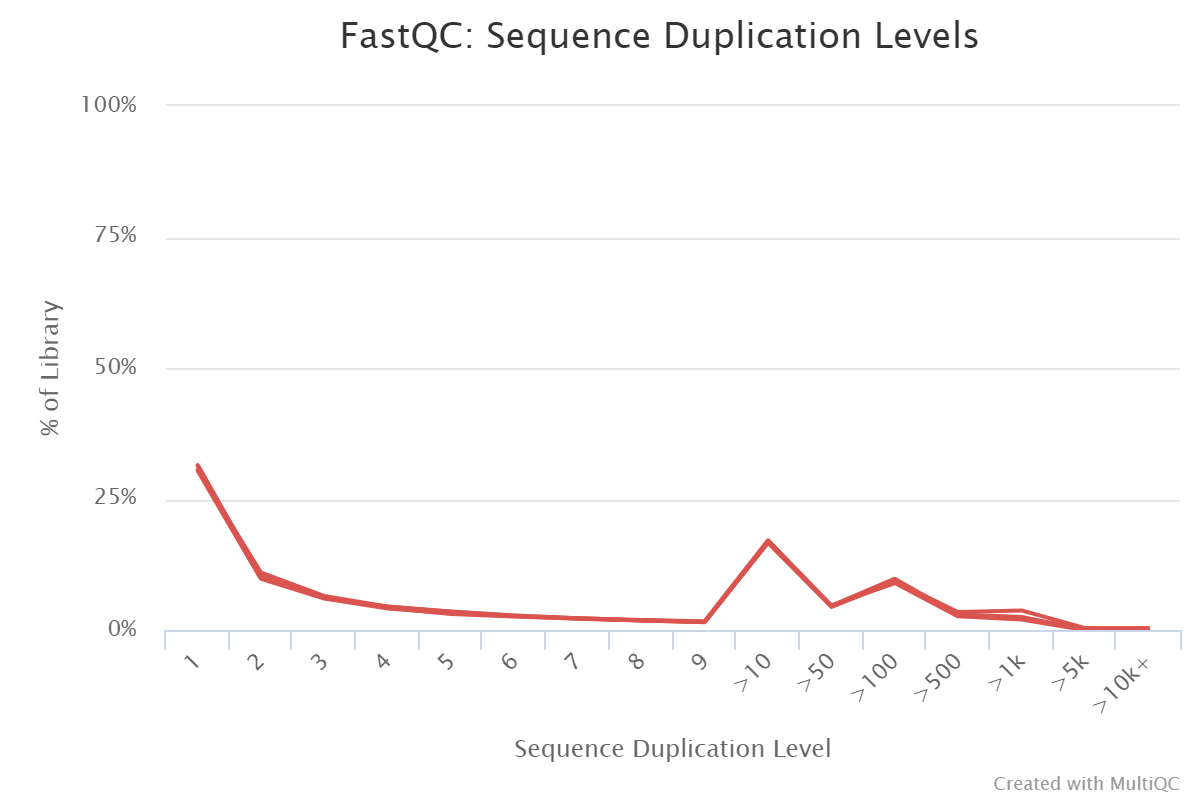
\includegraphics[width=1\textwidth]{fastqc_sequence_duplication_levels_plot}
    \caption[Sequence duplication levels plots for all samples]{Sequence duplication levels plots for all samples, showing the wide range of possible coverages in RNA data, ranging from 1 to >10,000.} 
    \label{fig:fastqc_sequence_duplication_levels_plot}
\end{figure}

\newpage
In Figure \ref{fig:fastqc_per_base_sequence_quality_plot}, sequence quality peaks at around the 14th base-pair, then gradually declines which is a classic sign of phasing. \cite{pfeiffer2018systematic} describe it as two similar phenomena: pre-phasing and post-phasing, both of which cause the reads to become out-of-sync. Pre-phasing occurs when two or more nucleotides bind to the read in a single cycle, causing the sequence to ‘skip’ a nucleotide. This often occurs when the flow-cell is not flushed properly or in the case of a defect terminator cap. Post-phasing is caused by the incomplete removal of the terminator cap, leading to the sequence lagging behind the rest of the cluster. As the number of cycles increases, the higher the probability of an error to occur which causes the read to become out of phase, and when this occurs, it will pollute the light signals of all subsequent cycles.


\begin{figure}[!h]
    \centering
    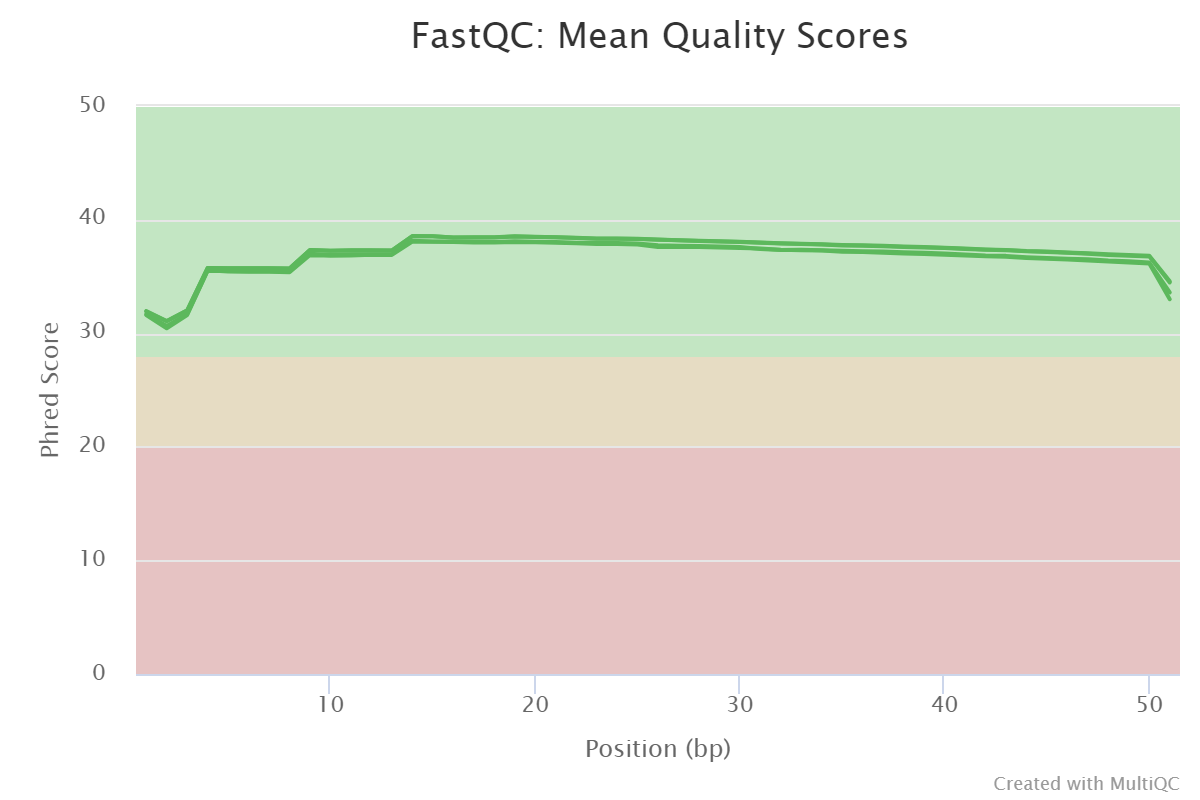
\includegraphics[width=1\textwidth]{fastqc_per_base_sequence_quality_plot}
    \caption{The aggregated mean Phred scores at each position of the reads.} % write about tpical pattern
    \label{fig:fastqc_per_base_sequence_quality_plot}
\end{figure}

\newpage
\autoref{fig:fastqc_per_sequence_gc_content_plot} shows a normal distribution which peaks around 48 \%GC, which is within the expected range for a human genome \citep{meunier2004recombination}. During PCR, endonucleases are less likely to cleave GC base pairs for two reasons: (i) their triple bond, which is stronger than the double bond in AT pairs, (ii) and because of  a phenomenon called base stacking which contributes to its structural stability \citep{yakovchuk2006base}. This may lead to GC-bias \citep{benjamini2012summarizing}, although this does not seem to be present.

\begin{figure}[!h]
    \centering
    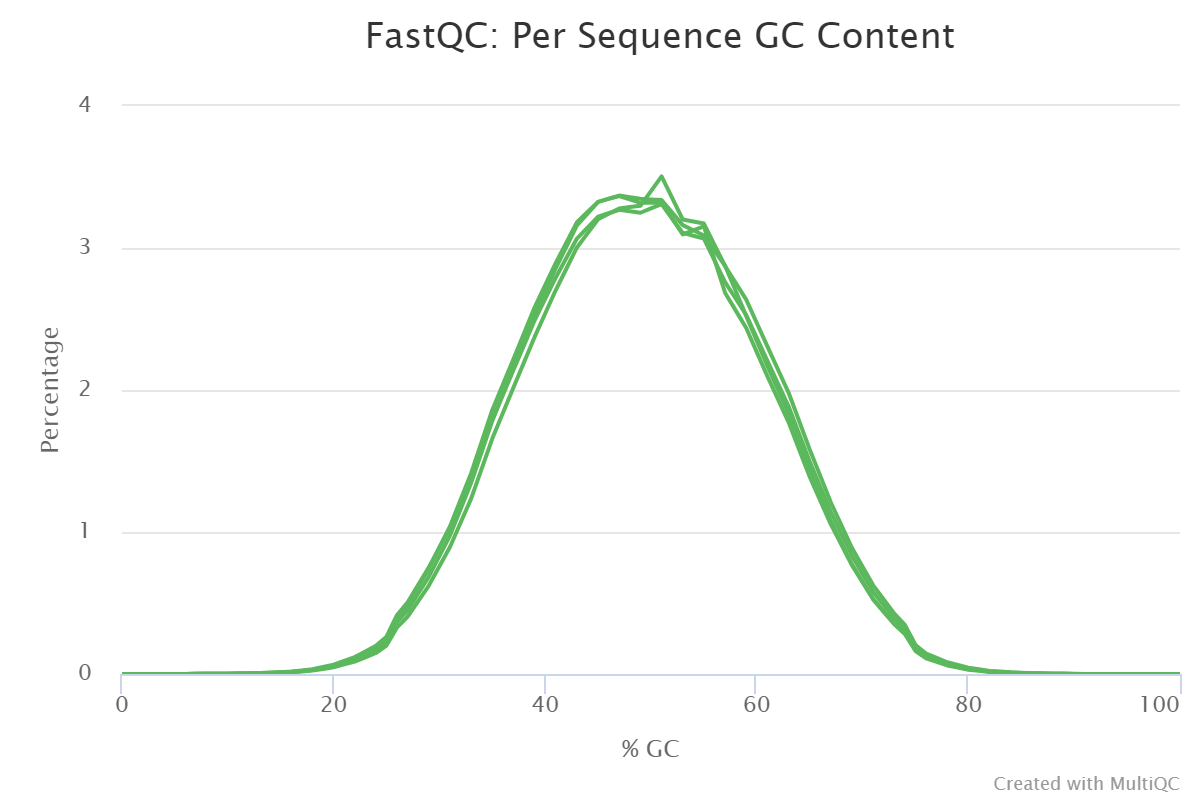
\includegraphics[width=1\textwidth]{fastqc_per_sequence_gc_content_plot}
    \caption{The distribution of GC percentages across the reads.}
    \label{fig:fastqc_per_sequence_gc_content_plot}
\end{figure}

\newpage
\autoref{fig:fastqc_per_sequence_quality_scores_plot} is similar to  \autoref{fig:fastqc_per_base_sequence_quality_plot}, except showing \textit{average} Phred scores on a sequence-level, instead of a base pair-level.


\begin{figure}[!h]
    \centering
    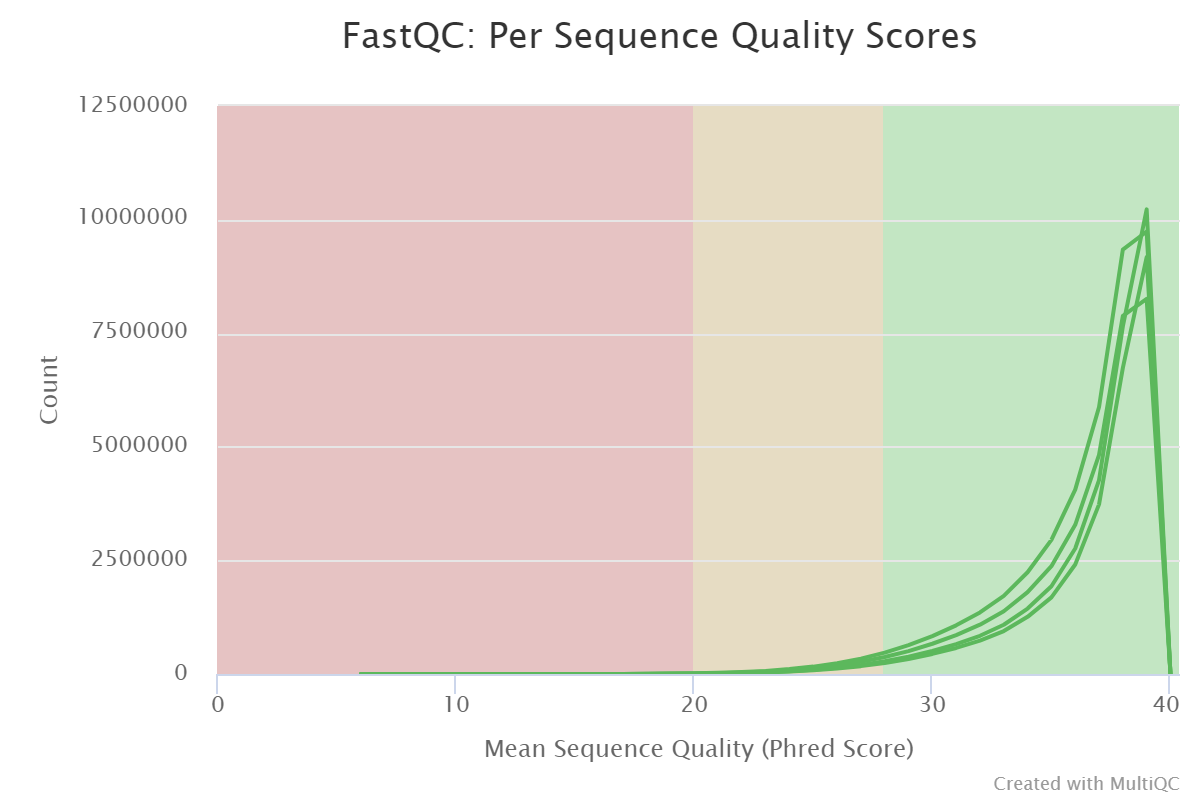
\includegraphics[width=1\textwidth]{fastqc_per_sequence_quality_scores_plot}
    \caption{The distribution of mean Phred scores across the reads.} % write about tpical pattern
    \label{fig:fastqc_per_sequence_quality_scores_plot}
\end{figure}

\newpage
Unequal read counts for each sample, as shown in \autoref{fig:fastqc_sequence_counts_plot} is expected in RNA-seq and is adjusted for in the downstream pipeline. As previously stated, the presence of duplicate reads is relatively benign in RNA-seq \citep{parekh2016impact}.


\begin{figure}[!h]
    \centering
    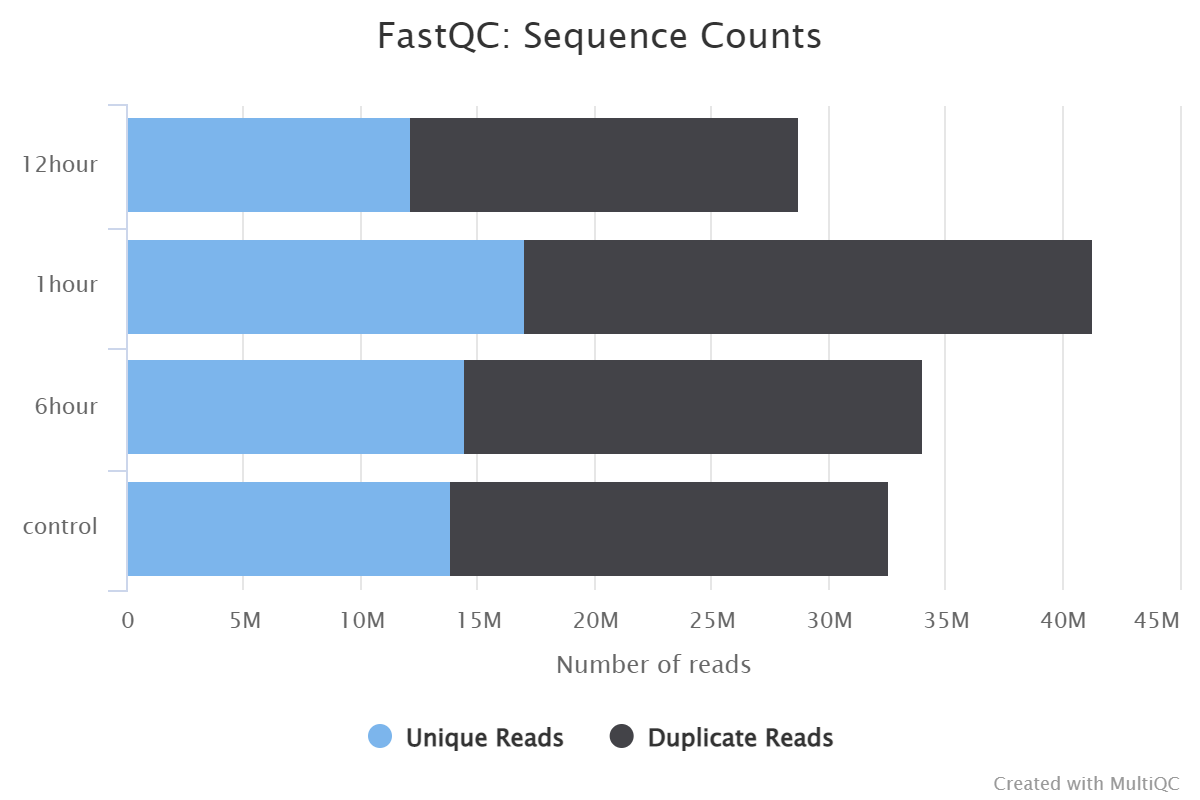
\includegraphics[width=1\textwidth]{fastqc_sequence_counts_plot}
    \caption{The number of reads for each sample, showing the proportion of duplicate reads.}
    \label{fig:fastqc_sequence_counts_plot}
\end{figure}
\newpage

The samples in \autoref{fig:fq_screen_plot} show no sign of contamination. There is an almost 100\% successful alignment to the human genome, with some alignment to other sequences which share genetic similarities. Some degree of multi-mapping (20\%) with the human reference is present. This may be caused by regions of low-complexity or by structural variants \citep{rhoads2015pacbio}

\begin{figure}[!h]
    \centering
    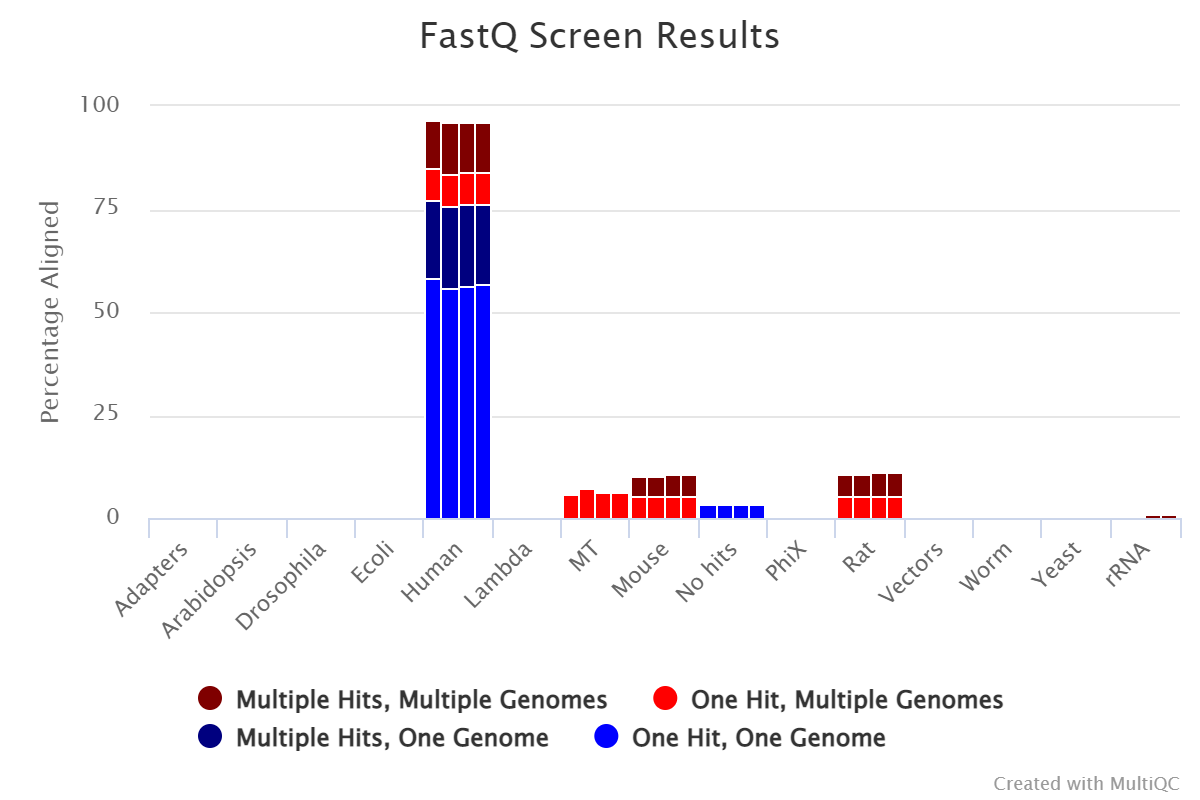
\includegraphics[width=1\textwidth]{fq_screen_plot}
    \caption{FastQ Screen plot showing the percentage of the reads aligned to which reference sequence(s).} 
    \label{fig:fq_screen_plot}
\end{figure}


\subsection{Preprocessing}
FastQC detected traces (<0.5\%) of TruSeq adapters in the FASTQ files, which is corroborated by the sequencer's manual \citep{HiSeq2000} stating that it makes use of the 'TruSeq family of reagents'. Adapter sequences were trimmed using CutAdapt (\autoref{fig:cutadapt_trimmed_sequences_plot_3}), and resultant reads shorter than 45 bp long were removed. Smaller reads lead to greater ambiguity during alignment as they have a greater probability of being multi-mapped.  The data was of good quality to begin with, so trimming had little overall effect on the reads, although the read lengths are no longer uniform.
%Between 1.3 and 1.6\% of all base-pairs were trimmed across the four samples. (why is this happening)


\begin{figure}[!h]
    \centering
    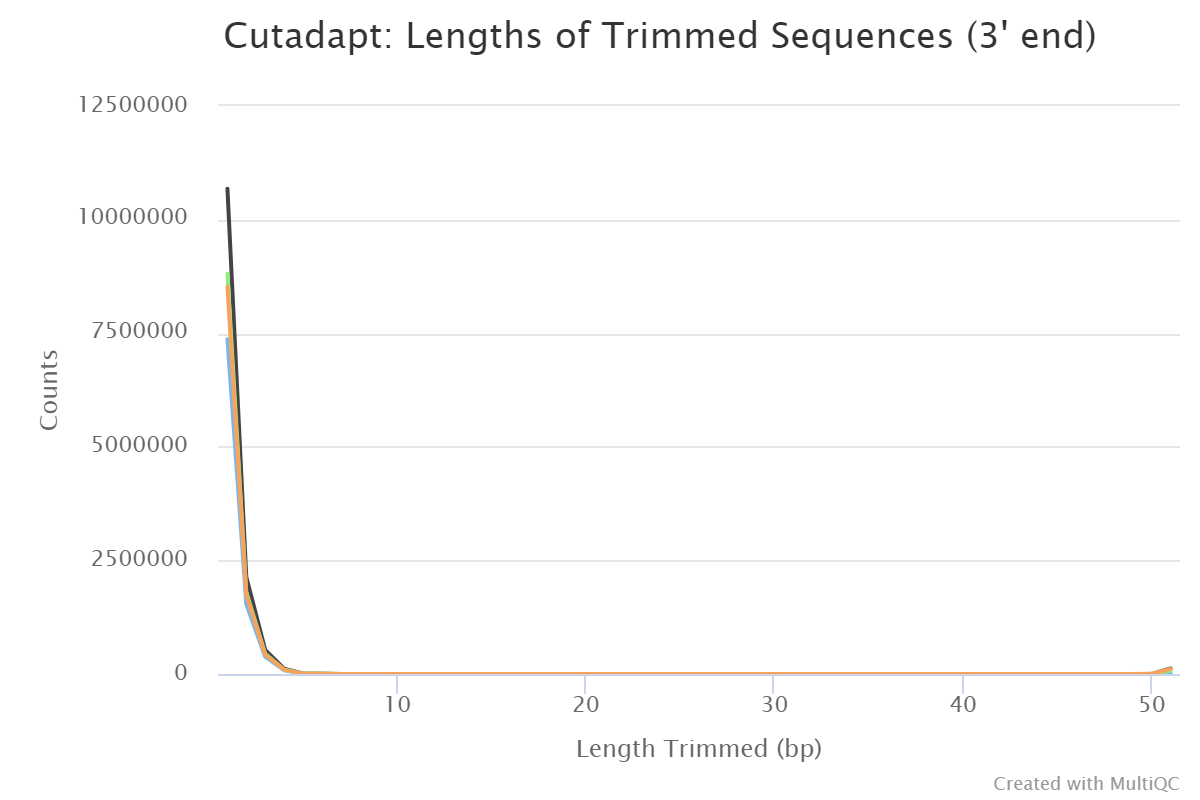
\includegraphics[width=1\textwidth]{cutadapt_trimmed_sequences_plot_3}
    \caption{The number of base-pairs trimmed per read from the 3' end.} 
    \label{fig:cutadapt_trimmed_sequences_plot_3}
\end{figure}
\newpage

MultiQC does not support Prinseq++ as of version 1.11, however its output reports are simple to interpret. They provide the number of reads filtered by \texttt{-lc\textunderscore dust} according to their DUST score (a measure of low complexity). These figures removed approximately 0.1\% of the total amount of reads for their respective sample. No reads were removed by \texttt{-ns\textunderscore max\textunderscore n} based on the number of \textit{N}'s.

%Control & 43764  \\ 
%        1 hour & 57736 \\ 
%        6 hour & 46910  \\ 
%        12 hour & 46369 \\ 


\subsection{Read Alignment}
The removal of short reads and reads low in complexity has reduced ambiguity when aligning to a reference genome \citep{rhoads2015pacbio}. Nonetheless STAR experienced some degree of multimapping, shown in \autoref{fig:star_alignment_plot}. The number of loci \texttt{Nmap} a read maps to is stored in the generated BAM file as \texttt{NH:i:Nmap}. If \texttt{Nmap} exceeds a certain threshold (10 by default) it will be labelled as 'mapped to too many loci' and excluded from the final BAM file. This is the most significant filtering step so far, removing 16\% to 18\% of the total read counts. Despite the loss of this substantial chunk of our reads, the main causes \citep{rhoads2015pacbio} for multi-mapping have been mitigated where possible: 
\begin{itemize}
\item[] Low-complexity regions were filtered in the previous step using Prinseq++.
\item[] Structural variants, while frequent in cancer-derived transcriptomes, are bypassed in STAR's splice-aware algorithm \citep{Dobin2013}, allowing different parts of the same read to map to distant genomic loci (possibly to different strands or chromosomes).
\item[] Longer read lengths and paired-end reads should reduce multi-mapping, although these factors were immutable at this stage.
\end{itemize}


\begin{figure}[!h]
    \centering
    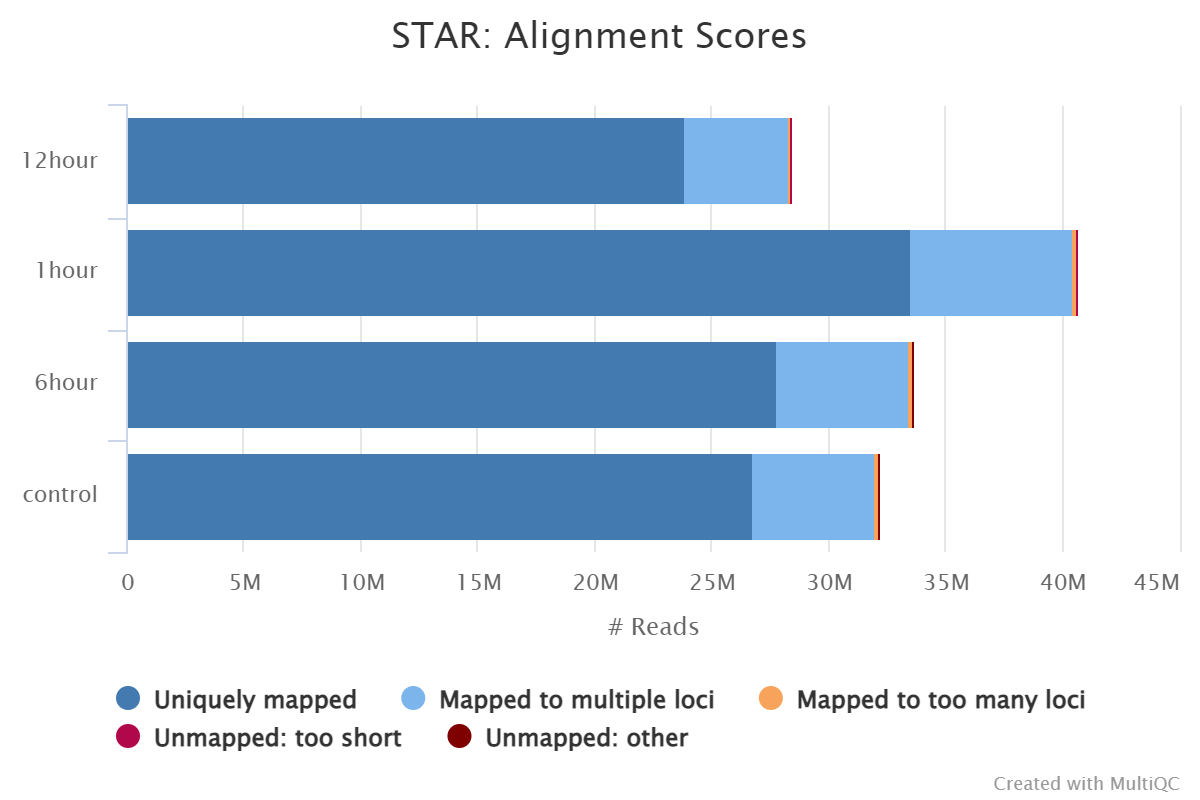
\includegraphics[width=1\textwidth]{star_alignment_plot}
    \caption{Number of uniquely mapped reads which passed all filters to the final BAM file, and the number of problematic reads which were consequently remained unaligned and were removed.} 
    \label{fig:star_alignment_plot}
\end{figure}
\newpage

%\subsection{Post-Alignment}
%At this stage tables containing information on the expected number of reads aligned to each gene are imported into R. Here we will be largely shifting our focus from the \textit{individual} reads, to \textit{collective} reads which align to each gene, i.e. to the expected read counts given in the tables produced through RSEM. The \ac{TMM} normalisation technique is performed, which adjusts the read count values per gene for confounding variables which are not biologically relevant. 

%Genes with low counts (<10) are removed as they can be considered as noise and are not expressed at any biologically meaningful level \citep{law2016rna}. These lowly expressed genes are particularly error-prone, and were shown to be highly sensitive to the \textit{in silico} methods used \citep{everaert2017benchmarking}.



\subsection{QC Summary}



The raw data in our starting FASTQ files was of good quality according to all tested metrics, resulting in Cutadapt and Prinseq++ having little effect on the read counts (\autoref{tab:read_counts}). Nonetheless a substantial portion of the reads suffered from multi-mapping and were removed.

\begin{table}[!h]
\centering
\caption{The resultant read counts after each data processing step.}
\label{tab:read_counts}
\begin{tabular}{cclll}
\toprule
                                                                   & \textbf{Control} & \textbf{1 hour} & \textbf{6 hour} & \textbf{12 hour} \\ \midrule
Raw data                                       & 32.62M           & 41.30M          & 34.08M          & 28.77M           \\ 
\begin{tabular}[c]{@{}c@{}}Trimming \\ (Cutadapt)\end{tabular} & 32.23M           & 40.81M          & 33.71M          & 28.54M           \\ 
\begin{tabular}[c]{@{}c@{}}Filtering\\ (Prinseq++)\end{tabular}    & 32.22M           & 40.75M          & 33.66M          & 28.50M           \\ 
\begin{tabular}[c]{@{}c@{}}Alignment \\ (STAR)\end{tabular}        & 26.80M           & 33.54M          & 27.78M          & 23.89M           \\ \bottomrule
\end{tabular}
\end{table}


% The edgeR vignette suggests to use the raw counts (?) of RSEM for normalisation, as opposed to using the already normalised TPM so we went with this.
 % FPKM/RPKM are not good measures of relative abundance because the FPKM/RPKM of a transcript can change between two samples even if its relative abundance stays the same.
% https://groups.google.com/g/rsem-users/c/GRyJfEOK1BQ <- very good explanation 

%\subsection{Multiple testing Correction}
%FDR
%Benjamini Hochback 


\section{Differential Gene Expression Analysis}

% Volcano plot
% Venn diagrams
% Sample heatmap
% Gene heatmap
% Cutoffs were largely arbitrary
%Discuss the FDR error rate. 5% of our DEGs are false positives





\subsection{Gene Set Enrichment Analysis}

%Pathview results
%GAGE: WTF DOES GAGE DO (check lit review)

\subsection{Evaluation of Results}
% List of DEGs from tyrosol study:  https://www.mdpi.com/2076-3417/11/21/10199
% House keeping genes
% Do the pathways make sense


% https://www.biostars.org/p/9510180/ reply says that even though a gene is downregulated, it might be suppressing other genes in the pathway which makes the other genes indirectly upregulated. Keep stuff like this in mind when interpreting gene expression.




% 1 hour was an outlier. Hypothesis: Cells which were differentiated died off (degrading their RNA) while others proliferated
% this is supported by the literature. Check if apoptosis pathways for the 6hr and 12hr are activated as opposed to differentiation pathways of the 1hr
% We dont know how long this differentiation > apoptosis thing takes. The 1hr might be in the middle of apoptosis and/or differentiation. 6hr and 12hr the cells might have stabilised. Check pathways to be sure. 

% Problems with the reference genome: https://genomebiology.biomedcentral.com/articles/10.1186/s13059-019-1774-4

\section{Summary}
\enlargethispage{\baselineskip} % so you do not get a single line in another page
